\chapter{Vergelykings en Ongelykhede}
\setcounter{figure}{1}
\setcounter{subfigure}{1}

\section{Oplos van Lineêre Vergelykings}
\nopagebreak
 $ \hspace{-5pt}\begin{array}{cccccccccccc}   
\includegraphics[width=0.75cm]{col11306.imgs/summary_fullmarks.png} &   
\includegraphics[width=0.75cm]{col11306.imgs/summary_video.png} &   \end{array} $ \hspace{2 pt}\raisebox{-5 pt}{} {(section shortcode: MG10068 )} \par 
           
Die eenvoudigste vergelyking om op te los is ’n lineêre vergelyking. ‘n Vergelyking word lineêr genoem indien
die hoogste mag van die veranderlike $1$ is. Die volgende is voorbeelde van lineêre
vergelykings:\par 


\begin{equation*}
\begin{array}{ccl}\hfill 2x+2& =& 1\hfill \vspace{6pt} \\
 \hfill \dfrac{2-x}{3x+1}& =& 2\hfill \vspace{6pt} \\
\hfill 4(2x-9)-4x&=&4-6x \hfill  \vspace{6pt}\\ 
\hfill \dfrac{2a-3}{3}-3a&=&\dfrac{a}{3} \hfill\\
\end{array}
\end{equation*}
In hierdie afdeling sal ons leer om te bepaal wat die waarde van ’n veranderlike moet wees om ’n vergelyking waar
te maak. Byvoorbeeld, watter waarde van $x$ maak beide kante van die baie eenvoudige vergelyking,$x+1=1$ waar. Die Oplossing is $x=0$.\par 
Aangesien die definisie van ’n lineêre vergelyking is dat die hoogste mag van die veranderlike een $1$ moet wees,
is daar hoogstens een oplossing of wortel vir die vergelyking.\par 
Hierdie afdeling berus op al die metodes wat ons reeds bespreek het: uitvermenigvuldiging van uitdrukkings met
hakies, groepering van terme en faktorisering.\par 

\begin{equation*}
  \begin{array}{ccll}\hfill 2x+2& =& 1\hfill \\ 
      \hfill 2x& =& 1-2\hfill & \mbox{(groepeer soortgelyke terme saam)}\hfill \\ 
      \hfill 2x& =& -1\hfill & \mbox{(vereenvoudig)}\hfill \\
\hfill x&=& -\frac{1}{2} & \mbox{(deel weerskante met $2$)} \hfill
  \end{array}
\end{equation*}

\begin{equation*}

\end{equation*}
Vervang  $x=-\frac{1}{2}$ in die oorspronklike vergelyking. Dan kry ons:

\begin{equation*}
    \begin{array}{ccl}\hfill \mbox{LHS}& =& 2x+2\hfill \\
	  & =& 2(-\frac{1}{2})+2\hfill \\
	  & =& -1+2\hfill \\
	  & =& 1\hfill \\
	  \hfill \mbox{RHS}& =& 1\hfill \\
    \end{array}
\end{equation*}
Daarom is $x = -\frac{1}{2}$ 'n ware oplossing

\Tip{Wanneer jy die oplossing van ’n vergelyking gevind het, vervang die oplossing
in die oorspronklike vergelyking om jou antwoord te bevestig.}

\subsection*{Metode: Oplos van Lineêre Vergelykings}

Die algemene stappe in die oplos van lineêre vergelykings is:
\begin{enumerate}[noitemsep, label=\textbf{\arabic*}. ] 
    \item Verwyder alle hakies in die vergelyking.
    \item "Dra" al die terme wat die veranderlike bevat "oor" na die linkerkant van die vergelyking, en alle konstante terme (die getalle) na die regterkant van die gelykaanteken. Hou in gedagte dat die teken van die terme sal verander van (+) na (−) of omgekeerd, soos hulle ’oor’ die gelykaanteken ’beweeg’.
    \item Groepeer alle soortgelyke terme saam en vereenvoudig so ver as moontlik.
\item Faktoriseer, indien nodig.
    \item Vind die oplossing en skryf die antwoord(e) neer.
    \item Stel die oplossing in die oorspronklike vergelyking in om die antwoord te bevestig.
\end{enumerate}

\Tip{die twee kante van 'n vergelyking moet altyd balanseer; wat jy doen aan die een kant moet jy doen aan die ander kant. 'n moontlike oplossing van NIE de vergelyking bevredig nie, is nie geldig nie.}

\setcounter{subfigure}{0}
\begin{figure}[H] % horizontal\label{m39241*equations-1}
\textnormal{Khan academy video on equations - 1}\vspace{.1in} \nopagebreak
\label{m39241*yt-media1}\label{m39241*yt-video1}
\raisebox{-5 pt}{ 
\includegraphics[width=0.5cm]{col11306.imgs/summary_www.png}} { (Video:  MG10069 )}
\vspace{2pt}   $\theta $
    &

\vspace{.1in}
\end{figure}       

    
\begin{wex}{Oplos van Lineêre Vergelykings}
{
Los op vir $x$: $15-2x=3$
}
{
\westep{herrangskik}

\begin{equation*}
    \begin{array}{cclc}\hfill 15-2x& =& 3\hfill & \\
	    \hfill -2x& =& 3-15\hfill & \hfill 
	    
    \end{array}
\end{equation*}

\westep{Vereenvoudig}
\begin{equation*}
    \begin{array}{cccc}\hfill -2x& =&-12\hfill & 
	    
    \end{array}
\end{equation*}

\westep{Deel weerskante met $-2$}
\begin{equation*}
    \begin{array}{cccc}\hfill x& =&6\hfill & 
	    
    \end{array}
\end{equation*}
\westep{Stel die oplossing in die oorspronklike vergelyking in om die antwoord te bevestig.}  

\begin{equation*}
\begin{array}{ccc}\hfill 15 - 2(6)& =& 3\hfill \\
 \hfill 15-12& =& 3\hfill \\
\hfill 3 &=& 3\hfill
\end{array}
\end{equation*}
Aangesien beide kante gelyk is, is die antwoord korrek
}
\end{wex}

\begin{wex}
{Solving linear equations }
{Solve for $x$: $4(2x-9)-4x=4-6x$}
{
\westep{brei die hakies uit en vereenvoudig}

\begin{equation*}
    \begin{array}{ccl}\hfill 4(2x-9)-4x& =& 4-6x\hfill  \\ 
	\hfill 8x-36-4x& =& 4-6x\hfill   \\ 
	\hfill 8x-4x+6x& =& 4+36\hfill  \\ 
	\hfill (8x-4x+6x)& =& (4+36)\hfill   \\   
	\hfill 10x& =& 40\hfill  
    \end{array}
\end{equation*}

\westep{Deel weerskante deur $10$}
\begin{equation*}
    \begin{array}{ccl}
	\hfill \dfrac{10}{10}x& =& \dfrac{40}{10}\hfill\\
	\hfill x& =& 4\hfill  
    \end{array}
\end{equation*}

\westep{Stel die oplossing in die oorspronklike vergelyking in}  

\begin{equation*}
    \begin{array}{ccl}\hfill 4[2(4)-9]-4(4)& =& 4-6(4)\hfill \\
	\hfill 4(8-9)-16& =& 4-24\hfill \\
	\hfill 4(-1)-16& =& -20\hfill \\
	\hfill -4-16& =& -20\hfill \\
	\hfill -20& =& -20\hfill 
    \end{array}
\end{equation*}
Aangesien beide kante gelyk is, is die antwoord korrek 
}
\end{wex}

\begin{wex}{Oplos van Lineêre Vergelykings}
{Los op vir $x$: $\dfrac{2-x}{3x+1}=2$} 
{
\westep{Ons begin deur weerskante van die vergelyking te vermenigvuldig met $(3x+1)$}
Omdat deling met $0$ ontoelaatbaar is, is daar ’n beperking op die waarde van ($x\neq -\frac{1}{3}$)

\begin{equation*}
    \begin{array}{ccll}\hfill \dfrac{2-x}{3x+1}& =& 2\hfill & \\
	\hfill (2-x)& =& 2(3x+1)\hfill & \\ 
    \end{array}
\end{equation*}

\westep{brei hakies uit en vereenvoudig}
\begin{equation*}
    \begin{array}{ccll}
	\hfill 2-x& =& 6x+2\hfill & \hfill \\ 
	\hfill -x-6x& =& 2-2\hfill & \hfill \\ 
	\hfill -7x& =& 0\hfill & \hfill
    \end{array}
\end{equation*}

\westep{Deel weerskante deur $-7$}
\begin{equation*}
    \begin{array}{ccll}

	\hfill x& =& \dfrac{0}{-7}\hfill & \\
	\hfill x& =& 0\hfill & \hfill 
    \end{array}
\end{equation*}
Let op dat $0$ gedeel deur enige ander getal is $0$.

\westep{Stel die oplossing in die oorspronklike vergelyking in:}

\begin{equation*}
    \begin{array}{ccc}\hfill \dfrac{2-(0)}{3(0)+1}& =& 2\hfill \vspace{6pt}\\
	\hfill 2& =& 2\hfill 
\end{array}
\end{equation*}
Aangesien weerskante gelyk is, is die antwoord korrek
}
\end{wex}


\begin{wex}
{Oplos van Lineêre Vergelykings}
{Los op vir $a$: $\dfrac{2a-3}{3}-3a=\dfrac{a}{3}$}
{
\westep{Ons begin deur elk van die terme in die vergelyking te ver-
menigvuldig met  $3$ en vervolgens te vereenvoudig.}  

\begin{equation*}
    \begin{array}{cccc}\hfill 2a-3 - 9a &= &a\hfill & \\ 
\hfill -7a - 3 &= &a\hfill & 
    \end{array}
\end{equation*}

\westep{herrangskik en vereenvoudig}
\begin{equation*}
    \begin{array}{cccc}\hfill -7a -a &= &3\hfill & \\ 
\hfill -8a &= &3\hfill & \\
    \end{array}
\end{equation*}

\westep{Deel weerskante deur $-8$} 
\begin{equation*}
    \begin{array}{cccc}\hfill a &= & -\dfrac{3}{8}\hfill & \\ 

    \end{array}
\end{equation*}

\westep{Stel die oplossing in die oorspronklike vergelyking in:}
\begin{equation*}
    \begin{array}{ccll}\hfill \dfrac{2(-\frac{3}{8}) - 3}{3} - 3(-\frac{3}{8}) &= & \dfrac{-\frac{3}{8}}{3}\hfill & \\ 
\\
      \hfill \dfrac{(-\frac{3}{4}) - \frac{12}{4}}{3} + \frac{9}{8} &= & \dfrac{-\frac{3}{8}}{3}\hfill & \\ 
\\
 \hfill \Bigg[-\frac{15}{4} \times \frac{1}{3}\Bigg] + \frac{9}{8} &= & -\frac{3}{8} \times \frac{1}{3}\hfill & \\ 
\\
 \hfill -\frac{5}{4} + \frac{9}{8} &= & -\frac{1}{8}\hfill & \\ 
 \hfill -\frac{10}{8} + \frac{9}{8} &= & -\frac{1}{8}\hfill & \\ 
 \hfill -\frac{1}{8} &= & -\frac{1}{8}\hfill & 
    \end{array}
\end{equation*}
Beide kante is gelyk, dus die oplossing is reg.
}
\end{wex}

\begin{exercises}{}
{
Oplos van Lineêre Vergelykings: \\
Assume all denominators are non-zero.
\begin{multicols}{2}
\begin{enumerate}[noitemsep, label=\textbf{\arabic*}. ] 
\item   $2y-3=7$
\item   $-3y=0$        
\item   $16y+4=-10$        
\item   $12y+0=144$
\item   $7+5y=62$   \vspace{6pt}     
\item  $55=5x+\dfrac{3}{4}$ \vspace{6pt}
\item   $5x=2x+45$        
\item  $23x-12=6+3x$
\item   $12-6x+34x=2x-24-64$
\item   $6x+3x=4-5(2x-3)$
\item   $18-2p=p+9$   \vspace{6pt}
\item   $\dfrac{4}{p}=\dfrac{16}{24}$
\item   $-(-16-p)=13p-1$
\item   $3f-10=10$
\item   $3f+16=4f-10$
\item   $10f+5=-2f-3f+80$
\item   $8(f-4)=5(f-4)$
\item  $6=6(f+7)+5f$      
\item $(a-1)^{2} - 2a = (a+3)(a-2) - 3$
\item $-7x = x+8(1-x)$ \vspace{6pt}
\item $5-\dfrac{7}{b} = \dfrac{2(b+4)}{b}$\vspace{6pt}
\item $\dfrac{x+2}{4} - \dfrac{x-6}{3} = \dfrac{1}{2}$\vspace{6pt}
\item $ 3 - \dfrac{y-2}{4} = 4$\vspace{6pt}
\item $ \dfrac{a+1}{a+2} = \dfrac{a-3}{a+1}$
  
\end{enumerate}
\end{multicols}
\par \raisebox{-0.2em}{
\includegraphics[height=1em]{../icons/www.eps}} Kry die oplossing met die kortkodes:
\par \begin{tabular}[h]{cccccc}
(1.) lcR  &  (2.) lcR  &  (3.) lcR  &  (4.) lcR  &  (5.) lcR  &  (6.) lcn  &  (7.) lcn  &  (8.) lcn  &  (9.) lcn  &  (10.) lcn  &  (11.) lcQ  &  (12.) lcQ  &  (13.) lcQ  &  (14.) lcQ  &  (15.) lcQ  &  (16.) lcU  &  (17.) lcU  &  (18.) lcU  &  (19.) lcU  &  (20.) lcU  & \end{tabular}
}
\end{exercises}

\section{Oplos van Kwadratiese Vergelykings}

 $ \hspace{-5pt}\begin{array}{cccccccccccc}   
\includegraphics[width=0.75cm]{col11306.imgs/summary_fullmarks.png} &   
\includegraphics[width=0.75cm]{col11306.imgs/summary_video.png} &   \end{array} $ \hspace{2 pt}\raisebox{-5 pt}{} {(section shortcode: MG10070 )}       \par
’n Kwadratiese vergelyking, is ’n vergelyking waar die mag van die veranderlike hoogstens
$2$ is. \\Die volgende is voorbeelde van kwadratiese vergelykings:\par 


\begin{equation*}
    \begin{array}{ccl}\hfill 2{x}^{2}+2x& =& 1\hfill \\
	\hfill 3{x}^{2}+2x-1&=&0 \\ 
	\hfill 0&=&-2{x}^{2}+4x-2\hfill 
    \end{array}
\end{equation*}

Kwadratiese vergelykings verskil van lineêre vergelykings daarin dat ’n lineêre vergelyking slegs een oplossing
het, terwyl ‘n kwadratiese vergelyking hoogstens 2 oplossings het. Daar is spesiale gevalle waar ’n kwadratiese
vergelyking slegs een oplossing het.

\begin{activity}{}
Oplos van Kwadratiese Vergelykings $x^{2}=16$ using the following three different methods:
\begin{enumerate}[noitemsep, label=\textbf{\arabic*}. ] 
\item Inspection (trial and error)
\item Taking the square root
\item Faktorisering
\end{enumerate}
(Let op, indien $a \times b = 0$ dan $a = 0$ of $b=0$)
\end{activity}

As jy ’n kwadratiese uitdrukking kan faktoriseer, is jy een stap weg daarvan om ’n kwadratiese vergelyking op
te los. Byvoorbeeld $2{x}^{2}-x-3 = 0$

kan geskryf word as $(x+1)(2x-3)=0$.


\subsection*{Metode: Oplos van Kwadratiese Vergelykings}
\begin{enumerate}[noitemsep, label=\textbf{\arabic*}. ] 
\item Skryf die vergelyking die vorm $ax^{2} +bx +c =0$.
\item Deel heel eerste die hele vergelyking deur enige gemene faktore van die koëffisiënte, ten einde ’n vergelyk-
ing te kry van die vorm $a{x}^{2}+bx+c=0$ waar $a$, $b$ en
$c$ geen gemeenskaplike faktore het nie.
\\Byvoorbeeld $2{x}^{2}+4x+2=0$ Kan geskryf word as
${x}^{2}+2x+1=0$ deur te deel met $2$.
\item Skryf $a{x}^{2}+bx+c=0$ in terme van sy faktore  $(rx+s)(ux+v)=0$.

\item Wanneer ons die vergelyking geskryf het in die vorm  $(rx+s)=0$ of $(ux+v)=0$, so $x = -\dfrac{s}{r}$ of $x=-\dfrac{v}{u}$ respectively.
\item Vervang elke moontlike waarde van die oplossing in die oorspronklike vergelyking in om te toets of dit ’n
geldige oplossing is.

\end{enumerate}

% \label{m39247*eip-388}
\setcounter{subfigure}{0}
\begin{figure}[H] % horizontal\label{m39247*equations-3}
\textnormal{Khan academy video on equations - 3}\vspace{.1in} \nSolve 
\label{m39247*yt-media3}\label{m39247*yt-video3}
\raisebox{-5 pt}{ 
\includegraphics[width=0.5cm]{col11306.imgs/summary_www.png}} { (Video:  MG10071 )}
\vspace{2pt}
\vspace{.1in}
\end{figure}

        
\begin{wex}
{Oplos van Kwadratiese Vergelykings }
{Los op vir $x$: $3{x}^{2}+2x-1=0$}
{
\westep{The equation is in the required form $ax{2} + bx + c = 0$}

\westep{Faktoriseer}
\begin{equation*}
(x+1)(3x-1)=0
\end{equation*}

\westep{Solve for both solutions}
We have
\begin{equation*}
     \begin{array}{ccc}\hfill x+1&=&0\hfill \\
	\hfill \therefore x&=&-1
    \end{array}
\end{equation*}

of
\begin{equation*}
     \begin{array}{ccc}\hfill 3x-1&=&0\hfill \\
	\hfill \therefore x&=&\frac{1}{3}
    \end{array}
\end{equation*}
\westep{As ons die antwoorde instel in die oorspronklike vergelyking in,
vind ons die vergelyking is waar vir beide antwoorde.}
\westep{Write final answer}
Die oplossing van $3{x}^{2}+2x-1=0$ is dus $x=-1$ of $x=\frac{1}{3}$.
}
\end{wex}


\begin{wex}{ Oplos van Kwadratiese Vergelykings }
{ Vind die wortels van die kwadratiese vergelyking  $0=-2{x}^{2}+4x-2$}
{
\westep{deel weerskante van die vergelyking deur $-2$}

\begin{equation*}
\begin{array}{ccc}\hfill -2{x}^{2}+4x-2& =& 0\hfill \\ \hfill {x}^{2}-2x+1& =& 0\hfill \end{array}
\end{equation*}

\westep{The equation is in the required form $ax{2} + bx + c = 0$}

\westep{Faktoriseer}
\begin{equation*}
\begin{array}{ccc} \hfill (x-1)(x-1) &=& 0 \hfill \\
\hfill (x-1)^{2} &=&0 \hfill 
\end{array}
\end{equation*}

\westep{ die kwadratiese uitdrukking ’n volkome vierkant}
Hierdie is a voorbeeld van 'n spesiale situasie waar daar net een oplossing vir die Kwadratiese Vergelykings is
\begin{equation*}
\begin{array}{ccc} \hfill x -1 &=& 0 \hfill \\
\hfill \therefore x &=&1 \hfill 
\end{array}
\end{equation*}

\westep{ As ons die antwoorde instel in die oorspronklike vergelyking in, vind ons die vergelyking is waar vir beide antwoorde.}

 
\westep{Write the final answer}
The solution to $0=-2{x}^{2}+4x-2$ is $x=1$.
}
\end{wex}


\begin{exercises}{ }
{
Oplos van Kwadratiese Vergelykings:
\begin{multicols}{2}
\begin{enumerate}[noitemsep, label=\textbf{\arabic*}. ] 
\item  $(3x+2)(3x-4)=0$
\item  $(5x-9)(x+6)=0$
\item  $(2y+3)(2y-3)=0$ 
\item  $(2x+1)(2x-9)=0$    
\item  $(4x)(x-3)=-9$       
\item  $20m+25{m}^{2}=0$
\item  $2{x}^{2}-5x-12=0$  
\item  $-75{x}^{2}+290x=240$
\item  $2x=\frac{1}{3}{x}^{2}-3x+14\frac{2}{3}$
\item  ${x}^{2}-4x=-4$      
\item  $-{x}^{2}+4x-6=4{x}^{2}-5x+3$       
\item  ${t}^{2}=3t$  
\item  ${x}^{2}-10x=-25$      
\item  ${x}^{2}=18$
\item  ${p}^{2}-6p=7$
\item  $4{x}^{2}-17x-77=0$
\item  $14{x}^{2}+5x=6$
\item  $2{x}^{2}-2x=12$              
\end{enumerate}
\end{multicols}
\par \raisebox{-0.2em}{
\includegraphics[height=1em]{../icons/www.eps}} Kry die oplossing met die kortkodes:
\par\begin{tabular}[h]{cccccc}
(1.) lcP  &  (2.) lcP  &  (3.) lcP  &  (4.) lcP  &  (5.) lcP  &  (6.) lcE  &  (7.) lcE  &  (8.) lcE  &  (9.) lcE  &  (10.) lcE  &  (11.) lcE  &  (12.) lcm  &  (13.) lcm  &  (14.) lcm  &  (15.) lcm  &  (16.) lcm  &  (17.) lcm  &  (18.) lcm  &  (19.) lcm  & \end{tabular}
}
\end{exercises}
% %          \section{ Exponential equations}
% %     \nopagebreak
% %             \label{m39253} $ \hspace{-5pt}\begin{array}{cccccccccccc}   
\includegraphics[width=0.75cm]{col11306.imgs/summary_fullmarks.png} &   \end{array} $ \hspace{2 pt}\raisebox{-5 pt}{} {(section shortcode: MG10072 )} \par 
% %     
% %     
\section{Solving simultaneous equations}
$ \hspace{-5pt}\begin{array}{cccccccccccc}   
\includegraphics[width=0.75cm]{col11306.imgs/summary_fullmarks.png} &   
\includegraphics[width=0.75cm]{col11306.imgs/summary_video.png} &   \end{array} $ \hspace{2 pt}\raisebox{-5 pt}{} {(section shortcode: MG10076 )} \par

Tot dusver het alle vergelykings slegs een onbekende veranderlike gehad wat ons moes vind.
Wanneer twee onbekendes bepaal moet word, het ons twee vergelykings nodig. Hierdie vergelykings word gelyktydige vergelykings
genoem. Die oplossing vir die stelsel van gelyktydige vergelykings is die waardes van die veranderlikes wat die stelsel van vergelykings gelyktydig sal bevredig. In die algemeen beteken dit indien daar $n$ onbekende veranderlikes is, benodig ons $n$ vergelykings om ’n oplossing vir elk van die $n$ veranderlikes te vind.\par 
’n Voorbeeld van stel gelyktydige vergelykings is:

\begin{equation*}
\begin{array}{rcl} x+y&=&-1 \\ 
 3&=&y-2x 
\end{array}
\end{equation*}

Om ’n numeriese waarde vir onbekende veranderlikes te vind, moet ons ten minste soveel onafhanklike vergelykings as veranderlikes hê. Ons kan gelyktydige vergelykings algebraïes of grafies oplos.\par 
\setcounter{subfigure}{0}
\begin{figure}[H] % horizontal\label{m39257*simultaneous-equations}
\textnormal{Khan academy video on simultaneous equations - 1}\vspace{.1in} \nopagebreak
\label{m39257*yt-media7}\label{m39257*yt-video7}
\raisebox{-5 pt}{ 
\includegraphics[width=0.5cm]{col11306.imgs/summary_www.png}} { (Video:  MG10077 )}
\vspace{2pt}
\vspace{.1in}
\end{figure}       

\subsection*{Oplossing deur Vervanging}
\begin{itemize}
 \item Probeer een van die vergelykings op te los vir een van die veranderlikes.
\item Vervang die resultaat in die ander vergelykings. Deur dit te doen verminder die hoeveelheid
vergelykings en ook die hoeveelheid onbekende veranderlikes met 1.
\item Hierdie proses word herhaal tot ‘n enkele vergelyking met 1 veranderlike oorbly, wat (hopelik) opgelos kan word.
\item Use the solution to substitute back into the first equation to find the value of the other unknown variable.
\end{itemize}

\Note{If the question does not explicitly ask for a graphical solution, then the system of equations should be solved algebraically.}

\begin{wex}
{Gelyktydige Vergelykings}
{
Los die volgende stelsel gelyktydige vergelykings op:
\begin{equation*}
\begin{array}{ccl}\hfill x-y& =& 1\hfill \\ \hfill 3& =& y-2x\hfill \end{array}
\end{equation*}
}
{
\westep{los ons die eerste vergelyking op vir $x$ in terme van $y$}
\begin{equation*}
    \begin{array}{ccl}\hfill x& =& y+1\hfill 
    \end{array}
\end{equation*}

\westep{en stel hierdie resultaat in die tweede vergelyking in: $y$}
\begin{equation*}
    \begin{array}{ccl}\hfill 3& =& y-2(y+1)\hfill \\
	\hfill 3& =& y - 2y - 2\hfill \\
	\hfill 5& =& -y\hfill \\
\hfill \therefore y& =& -5\hfill
    \end{array}
\end{equation*}

\westep{vervang nou dit treug in die oorspronklike vergelyking in en solvelos op vir $x$}
\begin{equation*}
    \begin{array}{ccl}\hfill x - (-5)& =& 1\hfill \\
	\hfill x+ 5& =& 1\hfill \\
\hfill \therefore x& =& -4\hfill
    \end{array}
\end{equation*}

\westep{Check the solution by substituting back into both original equations}  

\westep{Write the final answer}
\begin{equation*}
\begin{array}{ccl}\hfill y& =& -5\hfill \\
 \hfill x& =& -4\hfill 
\end{array}
\end{equation*}
}
\end{wex}

\begin{wex}
{gelyktydige vergelykings}
{
los die volgende stelsel gelyktydige vergelykings op:
\begin{equation*}
\begin{array}{ccc}\hfill 4y+3x& =& 100\hfill \\ 
\hfill 4y - 19x& =& 12\hfill 
\end{array}
\end{equation*}
}
{
\westep{Use either equation to express $x$ in terms of $y$}
\begin{equation*}
    \begin{array}{ccl}\hfill 4y+3x & =& 100\hfill \\
\hfill 3x &=& 100 - 4y \hfill \\
\hfill x& =& \dfrac{100 - 4y}{3} \hfill
    \end{array}
\end{equation*}


\westep{Substitute into the second equation and solve for $y$}
\begin{equation*}
    \begin{array}{ccl}\hfill 4y - 19(\dfrac{100 - 4y}{3})& =& 12\hfill \\
	\hfill 12y - 19(100 - 4y)  & =& 36\hfill \\
	\hfill 12y - 1900 + 76y & =& 36 \hfill \\
\hfill  88y& =& 1936 \hfill \\
\hfill \therefore y& =& 22 \hfill
    \end{array}
\end{equation*}

\westep{Substitute back into the first equation and solve for $x$}
\begin{equation*}
    \begin{array}{ccl}\hfill x &=& \dfrac{100 - 4(22)}{3}\hfill \vspace{6pt}\\
	\hfill & =& \dfrac{100-88}{3}\hfill \vspace{6pt}\\
	\hfill & =& \dfrac{12}{3}\hfill\vspace{6pt} \\
	\hfill \therefore x&=& 4 \hfill 
    \end{array}
\end{equation*}

\westep{Check the solution by substituting back into both original equations}  

\westep{Write the final answer}
\begin{equation*}
\begin{array}{ccc}
 \hfill x& =& 4\hfill \\
\hfill y& =& 22\hfill 
\end{array}
\end{equation*}
}
\end{wex}

\subsection*{Solving by elimination}

\begin{wex}
{Simultaneous equations }
{
Solve the following system of equations:
\begin{equation*}
\begin{array}{ccll}\hfill & 3x+y& =& 2\hfill \\ 

\hfill& 6x-y& =& 25\hfill 
\end{array}
\end{equation*}
}
{
\westep{Make the coefficients of either variable in both equations the same}
The coefficients of $y$ in the given equations are $1$ and $-1$. Eliminate the variable $y$ by adding the two equations together
\begin{equation*}
\begin{array}{ccll}\hfill & 3x+y& =& 2\hfill \\ 
\hfill+ & 6x-y& =& 25\hfill \\ \hline
 \hfill & 9x + 0 &=& 27
\end{array}
\end{equation*}


\westep{vereenvoudig en los op vir $x$}
\begin{equation*}
    \begin{array}{ccl}\hfill 9x& =& 27\hfill \\
	\hfill \therefore x  & =& 3\hfill 
    \end{array}
\end{equation*}

\westep{Substitute the value of $x$ back into either original equation and solve for $y$}
\begin{equation*}
    \begin{array}{ccl}\hfill 3(3) + y &=& 2\\
	\hfill y & =& 2-9\\
	\hfill \therefore y & =& -7 
   \end{array}
\end{equation*}

\westep{Check the solution $x=3$ and $y=-7$ satisfies both original equations}  

\westep{Write the final answer}
\begin{equation*}
\begin{array}{ccc}
 \hfill x& =& 3\hfill \\
\hfill y& =& -7\hfill 
\end{array}
\end{equation*}
}
\end{wex}

\begin{wex}
{Simultaneous equations }
{
Solve the following system of equations:
\begin{equation*}
\begin{array}{cccc}\hfill & 2a - 3b& =& 5\hfill \\ 
\hfill& 3a-2b& =& 20\hfill 
\end{array}
\end{equation*}
}
{
\westep{Make the coefficients of either variable in both equations the same}
By multiplying the first equation by $3$ and the second equation by $2$, both coefficients of $a$ will be $6$.
\begin{equation*}
\begin{array}{cccc}\hfill & 6a-9b& =& 15\hfill \\ 
\hfill- & (6a-4b& =& 40)\hfill \\ \hline
 \hfill & 0 - 5b &=& -25 

\end{array}
\end{equation*}
(When subtracting two equations, be careful of the signs.)

\westep{Simplify and solve for $x$}
\begin{equation*}
    \begin{array}{ccl}
 \hfill b &=& \dfrac{-25}{-5} \\
 \hfill \therefore b &=& 5
    \end{array}
\end{equation*}

\westep{Substitute the value of $b$ back into either original equation and solve for $a$}
\begin{equation*}
    \begin{array}{ccl}\hfill 2a - 3(5)&=& 5\\
	\hfill 2a-15 & =& 5\\
	\hfill 2a & =& 20\\
	\hfill \therefore a & =& 10 
   \end{array}
\end{equation*}

\westep{Check the solution $a=10$ and $b=5$ satisfies both original equations}  

\westep{Write the final answer}
\begin{equation*}
\begin{array}{ccc}
 \hfill a& =& 10\hfill \\
\hfill b& =& 5\hfill 
\end{array}
\end{equation*}
}
\end{wex}


\subsection*{Solving graphically}

Gelyktydige vergelykings kan grafies opgelos word. Die oplossing van die gelyktydige vergelykings word gegee
deur die koördinate van die punt waar die twee grafieke mekaar sny.\par 
For example:
\begin{equation*}
\begin{array}{cc}\hfill x=2y\\ \hfill y=2x-3\end{array}
\end{equation*}

Skets die grafieke van die 2 vergelykings in.\par 

\setcounter{subfigure}{0}
\begin{figure}[H] % horizontal\label{m39257*uid96}
\begin{center}
\rule[.1in]{\figurerulewidth}{.005in} \\
\label{m39257*uid96!!!underscore!!!media}\label{m39257*uid96!!!underscore!!!printimage}
%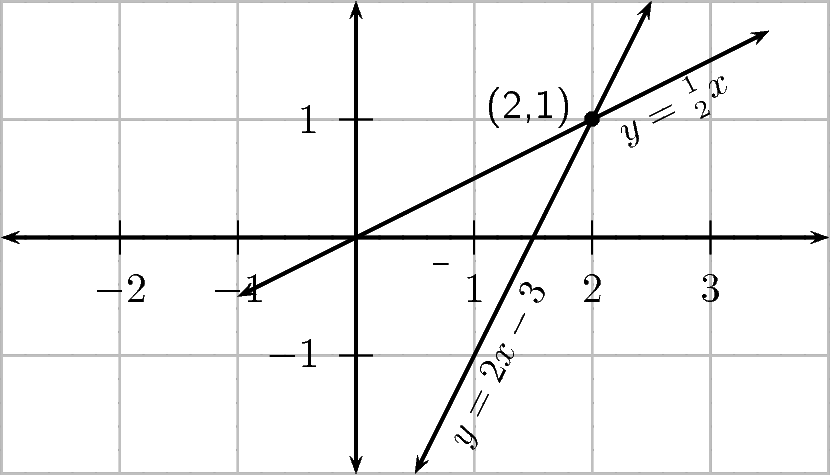
\includegraphics[width=.8\columnwidth]{col11306.imgs/m39257_MG10C10_006.png} % m39257;MG10C10\_006.png;;;6.0;8.5;
\begin{pspicture}(-3,-2)(4,2)
% \psgrid[gridcolor=lightgray,gridlabels=0,gridwidth=0.5pt]
\psaxes[dx=1,Dx=1,arrows=<->](0,0)(-3,-2)(4,2)
\pstextpath[c](-1.1,-0.3){\psplot[xunit=1,plotstyle=curve,arrows=<->]{0.5}{2.5}{x 2 mul 3 sub}}{\small{$y=2x-3$}}
\pstextpath[c](1.5,-0.3){\psplot[xunit=1,plotstyle=curve,arrows=<->]{-1}{3.5}{0.5 x mul}}{\small{$y=\frac{1}{2}x$}}
\uput[l](2,1.1){$(2,1)$}
\psdot(2,1)
\end{pspicture}

\vspace{2pt}
\vspace{.1in}
\rule[.1in]{\figurerulewidth}{.005in} \\
\end{center}
\end{figure}       
Die snypunt van die 2 grafieke is $(2;1)$. Dus, die oplossing van die stel gelyktydige vergelykings in $x=2$ en $y=1$.\par 
Dit kan algebraïes getoon word as. \\
Stel die eerste vegelyking in die tweede vergelyking in:

\begin{equation*}
\begin{array}{ccl}\hfill x& =& 2y\hfill \\
 \hfill y& =& 2(2y)-3\hfill 
\end{array}
\end{equation*}
Los op vir $y$:
\begin{equation*}
\begin{array}{ccl}
 \hfill y-4y& =& -3\hfill \\
 \hfill -3y& =& -3\hfill \\ 
\hfill \therefore y& =& 1\hfill 
\end{array}
\end{equation*}
Stel die antwoord vir $y$ in die eerste vergelyking in:
\begin{equation*}
\begin{array}{ccl}
 \hfill x& =& 2(1)\hfill \\
 \therefore x&=& 2\hfill \end{array}
\end{equation*}

Notice that both methods give us the same solution.

\begin{wex}
{Gelyktydige vergelykings }
{Los die volgende stel gelyktydige vergelykings grafies op:
\begin{equation*}
\begin{array}{ccl}\hfill 4y+3x& =& 100\hfill \\ \hfill 4y-19x& =& 12\hfill \end{array}
\end{equation*}
}
{
\westep{Skryf alby vergelykings in die vorm $y=mx+c$}  

\begin{equation*}
\begin{array}{ccl}\hfill 4y+3x& =& 100\hfill \\
 \hfill 4y& =& 100-3x\hfill \\
 \hfill y& =& -\dfrac{3}{4}x + 25\hfill \end{array}
\end{equation*}
\\
\begin{equation*}
\begin{array}{ccl}\hfill 4y-19x& =& 12\hfill \\ \hfill 4y& =& 19x+12\hfill \\ \hfill y& =& \dfrac{19}{4}x+3\hfill \end{array}
\end{equation*}



\westep{Skets die grafieke van die 2 vergelykings in}
\setcounter{subfigure}{0}
\begin{figure}[H] % horizontal\label{m39257*id159679}
\begin{center}
\label{m39257*id159679!!!underscore!!!media}\label{m39257*id159679!!!underscore!!!printimage}
%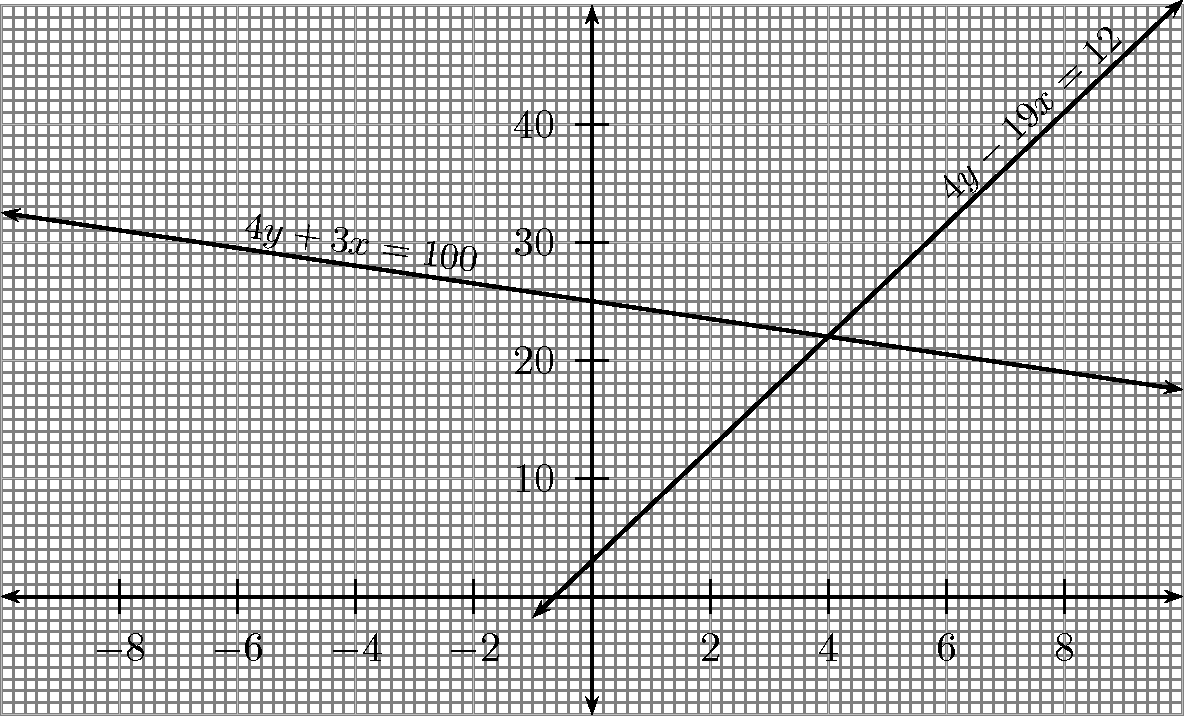
\includegraphics{col11306.imgs/m39257_MG10C10_007.png} % ;MG10C10\_007.png;;;6.0;8.5;
\begin{center}
\begin{pspicture}(-5,-1)(5,5)
%  \psgrid[subgriddiv=10,gridcolor=lightgray,gridlabels=0,gridwidth=0.1pt]
\psaxes[dx=1,dy=1,Dy=10,Dx=2,arrows=<->](0,0)(-5,-1)(5,5)
\pstextpath[c](-2,0.1){\psplot[xunit=0.5,yunit=0.1,plotstyle=curve,arrows=<->]{-10}{10}{0.75 x mul neg 25 add}}{\small{$4y+3x=100$}}
\pstextpath[c](2.2,0.1){\psplot[xunit=0.5,yunit=0.1,plotstyle=curve,arrows=<->]{-1}{10}{4.75 x mul 3 add}}{\small{$4y-19x=12$}}
\end{pspicture}
\end{center}

\vspace{2pt}
\vspace{.1in}
\end{center}
\end{figure}         

\westep{Vind die snypunt van die twee grafieke}
The two graphs intersect at $(4;22)$ 

\westep{Write the final answer}
\begin{equation*}
\begin{array}{ccl}\hfill x& =& 4\hfill \\ \hfill y& =& 22\hfill \end{array}
\end{equation*}

}
\end{wex}

\begin{exercises}{}
{
 \Note{Solving a system of simultaneous equations graphically is sometimes not very accurate but provides a valuable method of solution.}
\item Los algebraïes op: 
\begin{enumerate}[noitemsep, label=\textbf{\arabic*}. ] 
\item $3x-14y=0$ , $x-4y+1=0$
\item $x+y=8$, $3x + 2y = 21$
\item $y=2x+1$ , $x + 2y + 3 = 0$
\end{enumerate}

Los grafies op en bevestig jou antwoord algebraïes::

\begin{enumerate}[noitemsep, label=\textbf{\arabic*}. ] 
\setcounter{enumi}{3}
\item  $x+2y=1$, $\frac{x}{3} + \frac{y}{2} = 1$
\item $5= x+y$ , $-x = y-2$
\item $3x - 2y = 0$ , $x - 4y + 1 = 0$

\end{enumerate}


\par \raisebox{-0.2em}{
\includegraphics[height=1em]{../icons/www.eps}} Kry die oplossing met die kortkodes:
\par \begin{tabular}[h]{cccccc}
(1.) lxq  &  (2.) lxl  &  (3.) lxi  &  (4.) lx3  & \end{tabular}
}
\end{exercises}

\section{Word problems}

$ \hspace{-5pt}\begin{array}{cccccccccccc}   
\includegraphics[width=0.75cm]{col11306.imgs/summary_fullmarks.png} &   \end{array} $ \hspace{2 pt}\raisebox{-5 pt}{} {(section shortcode: MG10079 )} \par

Die doel van hierdie afdeling is om vir jou die vaardighede te leer om ’n probleem te neem en dit wiskundig te
formuleer sodat dit opgelos kan word.


\subsection*{Probleemoplossing Strategie}

\begin{enumerate}[noitemsep, label=\textbf{\arabic*}. ] 
\item Lees die HELE vraag!
\item Bepaal wat gevra word.
\item Gebruik (’n) veranderlike(s) om die onbekende getalle/hoeveelhede wat gevra word voor te stel, byvoor-
beeld, $x$.
\item  Herskryf die inligting wat gegee is in terme van die veranderlike(s). Dus, vertaal die woorde in algebraïese
taal.
\item Stel ’n vergelyking of ’n stel gelyktydige vergelykings (’n Wiskundige model) op om die onbekende te kry.
\item Los die vergelyking algebraïes op om die oplossing te vind.
\item Toets die oplossing
\end{enumerate}

\begin{wex}
{Solving word problems}
{
 ’n Winkel verkoop tweewielfietse en driewiele. In totaal is daar $7$ etse (fietse sluit tweewielfietse en driewiele in) en $19$ wiele. Bepaal hoeveel van elke soort fiets is daar.
}
{
\westep{Assign variable to unknown}
as $b$ die aantal tweewielfietse en  \\
en laat $7-b$  die aantal driewiele is, dan: 

\westep{Set up an equation}
\begin{equation*}
\begin{array}{ccc}\hfill 2b+3(7-b)& =& 19\hfill \end{array}
\end{equation*}


\westep{Rearrange and solve for $b$}
\begin{equation*}
\begin{array}{ccl}
 \hfill 2b + 21 - 3b& =& 19\hfill \\
\hfill - b& =& -2\hfill \\
 \hfill \therefore b& =& 2\hfill 
\end{array}
\end{equation*}

\westep{Calculate number of tricycles}
\begin{equation*}
\begin{array}{ccl}
\\ \hfill  7 - 2 & =& 5\hfill \\
 \therefore \mbox{ Number of tricycles }& =& 5
\end{array}
\end{equation*}

\westep{Write final answer}
 There are $5$ tricycles and $2$ bicycles.

}       
\end{wex}

\begin{wex}{Solving word problems}{
Bongani and Jane are friends. Bongani takes Jane's physics test paper and will not tell her what her mark is. 
He knows that Jane hates maths so he decides to tease her. Bongani says: 'I have $2$ marks more than you do and the sum of both our marks is equal to $14$. 
How much did we get?'}
{
\westep{Assign variables to the unknowns}
We have two unknowns, Bongani's mark and
 Jane's mark. 
\\Let Bongani's mark be $t$ and Jane's mark be $j$. 

\westep{Set up a system of equations}
\\Bongani has $2$ more marks than Jane.
\begin{equation*}
t=j+2
\end{equation*}

Both marks add up to $14$.

\begin{equation*}
t+j=14
\end{equation*}

\westep{Use the first equation to express $t$ in terms of $j$}
\begin{equation*}
t=j+2
\end{equation*}

\westep{Substitute into second equation}
\begin{equation*}
    \begin{array}{ccc}\hfill t+j& =& 14\hfill \\
	\hfill (j+2)+j& =& 14\hfill \\

    \end{array}
\end{equation*}

\westep{Rearrange and solve for $j$}
\begin{equation*}
    \begin{array}{ccl}\hfill 2j& =& 14 - 2\hfill \\
	\hfill \therefore 2j& =& 12\hfill \\
\hfill \therefore j &=& 6 \hfill

    \end{array}
\end{equation*}

 \westep{Substitute value for $j$ back into first equation and solve for $t$}
\begin{equation*}
\begin{array}{ccl}\hfill t& =& j+2\hfill \\ & =& 6+2\hfill \\ & =& 8\hfill \end{array}
\end{equation*}
\\
\westep{Check the solution satisfies both original equations}
\westep{Write the final answer}
Bongani got $8$ for his test and Jane got  $6$.\\
}
\end{wex}

\begin{wex}
{Wiskundige Modellering}
{
’n
Vrugteskommel kos R$~2,00$ meer as ’n sjokolade melkskommel. As $3$ vrugteskommels en $5$ sjokolade melkskommels saam  R$~78,00$, kos,
bepaal die individuele pryse.}

{
\westep{Assign variables to unknowns}  
Gestel die prys van ’n sjokelade melkskommel is $x$ 
\\ rand en die prys van ’n vrugteskommel is  $y$ rand.


\westep{Set up a system of equations}
\begin{equation*}
\begin{array}{ccl} \hfill y &=& x+2 \hfill \\
\hfill 3y+5x& =& 78\hfill 
\end{array}
\end{equation*}

\westep{Substitute first equation into the second}
\begin{equation*}
\begin{array}{ccl}\hfill 3(x+2)+5x& =& 78\hfill \\
\end{array}
\end{equation*}

\westep{Rearrange and solve for $x$}
\begin{equation*}
\begin{array}{ccl}
 \hfill 3x+6+5x& =& 78\hfill \\ 
\hfill 8x& =& 72\hfill \\ 
\hfill \therefore x& =& 9\hfill \\  \end{array}
\end{equation*}

\westep{Substitute value for $x$ back into first equation and solve for $y$}
\begin{equation*}
\begin{array}{ccl}
\hfill y& =& x+2\hfill \\
 \hfill & =& 9+2\hfill \\ 
\hfill & \therefore =& 11\hfill  \end{array}
\end{equation*}
\westep{Check the solution satisfies both original equations}
\westep{Write final answer}
Een sjokelade melkskommel kos R$~9,00$ en een vrugteskommel
kos R$~ 11,00$.
}
\end{wex}

\begin{wex}
{Solving word problems }
{
The product of two consecutive negative integers is $1122$. Find the two integers.
} 
{
\westep{Assign variable to unknown}
Let the first integer be $n$ 
\\and let the second integer be $n+1$.\par 

\westep{Set up an equation}  
\begin{equation*}
\begin{array}{cll}\hfill n(n+1)& =& 1122\hfill \end{array}
\end{equation*}

\westep{Expand and solve for $n$}
\begin{equation*}
    \begin{array}{cll}
	\hfill n^{2} + n =& 1122\hfill \\
\hfill n^{2} + n - 1122 =& 0\hfill \\
\hfill (n+34)(n-33) =& 0\hfill \\
	\hfill \therefore  n =& -34 \hfill \\
\hfill \mbox{ or } n =& 33\hfill 
    \end{array}
\end{equation*}

\westep{Integers must be negative}
\begin{equation*}
    \begin{array}{cll}
	\hfill \therefore n =& -34\hfill \\
\hfill n + 1 =& -34\ + 1 \hfill \\
\hfill  =& -33\hfill \\

    \end{array}
\end{equation*}

\westep{Write final answer} 
The two consecutive negative numbers are $-34$ and $-33$.
}
\end{wex}

\begin{exercises}{Word problems}
{
\begin{enumerate}[noitemsep, label=\textbf{\arabic*}. ] 
\item Two jets are flying towards each other from airports that are $1~200$ km apart. One jet is flying at $250$ km/h and the other jet at $350$ km/h. If they took off at the same time, how long will it take for the jets to pass each other?
\item Kadesh bought $20$ shirts at a total cost of R$~980$. If the large shirts cost R$~50$ and the small shirts cost R$~40$, how many of each size did he buy?
\item Die diagonaal van ’n reghoek is $25~$cm meer as die wydte. Die lengte van die reghoek is $17~$cm meer as die wydte. Wat is die afmetings van die reghoek?  
\item Die som van $27$ en $12$ is gelyk aan $73$ meer as ’n onbekende getal. Vind die onbekende getal
\item Die twee kleiner hoeke van ’n reghoekige driehoek is in die verhouding $1:2$. Wat is die groottes van die
twee hoeke?
\item The length of a rectangle is twice the breadth. If the area is $128$ cm$^{2}$, determine the length and the breadth.       
\item As $4$ keer ’n getal met $7$, vermeerder word, is die resultaat $15$ minder as die vierkant (kwadraat) van die
getal. Vind die getal wat hierdie stelling bevredig deur ’n vergelyking op te stel en dan op te los.
\item Die lengte van ’n reghoek is $2~$cm cm meer as die wydte van die reghoek. Die omtrek van die reghoek is  $20~$cm. Vind die lengte en breedte van die reghoek.
\item Vian het $1~l$ liter van ’n mengsel wat $69\%$ out bevat. Hoeveel water moet Vian bygooi om die mengsel $50\%$ sout te maak? Skryf jou antwoord as ’n breukdeel van ’n liter.
       
\end{enumerate}

\par \raisebox{-0.2em}{
\includegraphics[height=1em]{../icons/www.eps}} Kry die oplossing met die kortkodes:
\par \begin{tabular}[h]{cccccc}
(1.) lcy  &  (2.) lcV  &  (3.) lcp  &  (4.) lcw  &  (5.) lcd  &  (6.) lcf  &  (7.) lcv  & \end{tabular}
}
\end{exercises}

\section{Vergelykings met Letterkoëffisiënte (Lettervergelykings)}
 $ \hspace{-5pt}\begin{array}{cccccccccccc}   
\includegraphics[width=0.75cm]{col11306.imgs/summary_fullmarks.png} &   \end{array} $ \hspace{2 pt}\raisebox{-5 pt}{} {(section shortcode: MG10078 )}\par
%   \label{m39258*eip-798}
%             \ssection{ Equations and inequalities: Literal equations}
%             \nopagebreak
%             

’n Vergelyking met letterkoëffisiënte is een wat verskeie letters of veranderlikes bevat. Voorbeelde sluit die area
van ’n sirkel($A=\pi{r}^{2}$) in en die formule vir die berekening van spoed ($s=\frac{d}{t}$). In hierdie afdeling sal jy leer hoe om vergelykings met letterkoëffisiënte op te los in terme van een van die veranderlikes. Om dit te doen, sal jy die beginsels oor die oplos van vergelykings wat jy geleer het, gebruik en toepas om die woordvergelykings te her-
rangskik. Die oplos van vergelykings met letterkoëffisiënte staan ook bekend as verandering van die onderwerp van ’n formule.
 
Wanneer jy lettervergelykings oplos, behoort jy die volgende in gedagte tehou:
\begin{itemize}
\item Ons isoleer die onbekende deur te vra wat daaraan verbind is en hoe dit daaraan verbind is en dan doen
ons die teenoorgestelde bewerking (aan beide kante as ’n geheel).
\item As die onbekende veranderlike in twee of meer terme voorkom, haal ons dit uit as ’n gemeenskaplike faktor. 
\item  As ons weerskante die vierkantswortel moet neem, onthou dat daar ’n positiewe sowel as ’n negatiewe
antwoord mag wees.
\item  As die onbekende veranderlike in die noemer is, dan vind ons die kleinste gemene noemer (KGN), ver-
menigvuldig weerskante met die KGN en gaan dan voort om die probleem op te los.
\end{itemize}


\begin{wex}
{Solving literal equations}
{
Die area van ’n driehoek is $A=\frac{1}{2}bh$. Wat is die hoogte van die driehoek in terme van die basis en area?
}
{
\westep{Isolate the required variable}
Ons herrangskik die vergelyking sodat die $h$ aan die een kant
van die gelykaanteken is en die res van die veranderlikes aan die
ander kant van die gelykaanteken.
\begin{equation*}
    \begin{array}{cccc}\hfill A& =& \frac{1}{2}bh\hfill & \\
	\hfill 2A& =& bh\hfill & \hfill \\
	\hfill \frac{2A}{b}& =& h\hfill 
    \end{array}
\end{equation*}

\westep{Write the final answer} 
Die hoogte van ’n driehoek word gegee deur: $h=\dfrac{2A}{b}$
} 
\end{wex}

\begin{wex}
{Oplos van Lettervergelykings}
{
Given the formula $h=\dfrac{H}{R+r} \times R$, solve for $R$.
}
{
\westep{Isolate the required variable}
\begin{equation*}
    \begin{array}{ccll}\hfill h(R+r)& =& H \times R\hfill & \\
	\hfill hR + hr& =& HR\hfill & \hfill \\
	\hfill hr & =& HR - hR\hfill \\
\hfill hr& =& R(H - h)\hfill \vspace{5pt}\\ 
\hfill \therfore R & =& \dfrac{hr}{H-h}\hfill 
    \end{array}
\end{equation*}

\westep{Write the final answer} 
$R = \dfrac{hr}{H-h}$
} 
\end{wex}


\begin{exercises}{}
{
\begin{enumerate}[noitemsep, label=\textbf{\arabic*}. ] 
\item Solve for $t$: $v=u+at$
\item Solve for $x$: $ax-bx=c$ \vspace{5pt}
\item Solve for $x$: $\dfrac{1}{b}+\dfrac{2b}{x}=2$\vspace{5pt}
\item Solve for $r$: $V = \pi r^{2} h$
\item Write $l$ in terms of $b$ and $H$: $\sqrt{l^{2}+b^{2}}=H$
\item Solve for $i$: $A=P(1+i)^{n}$
\item Solve for $h$: $A=2\pi rh + 2 \pi r$
\item Solve for $b$: $V=l \times b \times h$
\item Solve for $h$: $V=\frac{1}{3}\pi r^{2}h$
\end{enumerate}

\par \raisebox{-0.2em}{
\includegraphics[height=1em]{../icons/www.eps}} Find the answers with the shortcodes:
\par \begin{tabular}[h]{cccccc}
(1.) lgw  &  (2.) lgw  &  (3.) lgw  & \end{tabular}
}
\end{exercises}

\section{Lineêre Ongelykhede}
\nopagebreak
$ \hspace{-5pt}\begin{array}{cccccccccccc}   
\includegraphics[width=0.75cm]{col11306.imgs/summary_fullmarks.png} &   
\includegraphics[width=0.75cm]{col11306.imgs/summary_video.png} &   \end{array} $ \hspace{2 pt}\raisebox{-5 pt}{} {(section shortcode: MG10073 )} \par 


\begin{activity}{Linear inequalities}
{
Stel die volgende voor op getallelyne and using interval notation:
\begin{enumerate}[noitemsep, label=\textbf{\arabic*}. ] 
\item $x<4$
\item $x\leq 4$
\item $x\geq 4$
\item $x>4$
\end{enumerate}
}
\end{activity}

’n Lineêre ongelykheid is soortgelyk aan ’n lineêre vergelyking aangesien die hoogste eksponent van die veranderlike $1$. is. Die volgende is voorbeelde van lineêre ongelykhede.\par 

\begin{equation*}
\begin{array}{ccc}\hfill 2x+2& \leq& 1\hfill \\ \hfill \dfrac{2-x}{3x+1}&\geq& 2\hfill \\ \hfill \frac{4}{3}x-6&<& 7x+2\hfill \end{array}
\end{equation*}
Die metodes wat gebruik word om lineêre ongelykhede op te los, is identies aan dié wat gebruik word om
lineêre vergelykings op te los. Die enigste verskil kom voor wanneer daar ’n vermenigvuldiging met of deling
deur ’n negatiewe getal is. Ons weet byvoorbeeld dat
t $8>6$. As beide kante van die ongelykheid gedeel word (byvoorbeeld deur  $-2$ sien ons $-4 > -3$ nie. Dus moet die ongelykheid omkeer, wat beteken
$-4<-3$.

\Tip{Wanneer beide kante van ’n ongelykheid met ’n negatiewe getal ver-
menigvuldig word, of met ’n negatiewe getal gedeel word, verander die rigting van
die ongelykheid. Om hierdie rede mag ons nie met ’n veranderlike vermenigvuldig as
ons nie weet nie wat die onbekende (veranderlike) se teken is nie.}

Byvoorbeeld, as  $x<1$, dan $-x>-1$.
Om ’n ongelykheid met ’n gewone vergelyking te vergelyk, sal ons eers die gewone vergelyking oplos. Los op $2x+2=1$.

\begin{equation*}
\begin{array}{ccl}\hfill 2x+2& =& 1\hfill \\ \hfill 2x& =& 1-2\hfill \\ \hfill 2x& =& -1\hfill \\ \hfill x& =& -\frac{1}{2}\hfill \end{array}
\end{equation*}
As ons hierdie antwoord op ’n getallelyn voorstel, kry ons:\par 

\setcounter{subfigure}{0}
\begin{figure}[H] % horizontal\label{m39254*id157630}
\begin{center}
\label{m39254*id157630!!!underscore!!!media}\label{m39254*id157630!!!underscore!!!printimage}
%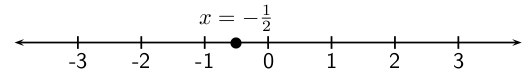
\includegraphics[width=.8\columnwidth]{col11306.imgs/m39254_MG10C10_001.png} % m39254;MG10C10\_001.png;;;6.0;8.5;
\begin{center}
\begin{pspicture}(-4,0.75)(4,1.75)
%\psgrid
\psline[arrows=<->](-4,1)(4,1)
\psdot[dotsize=5pt](-0.5,1)
\multido{\n=-3+1}{7}
{\uput[d](\n,1){$\n$}
\psline(\n,1.1)(\n,0.9)}
\uput[u](-0.5,1){$x=-\frac{1}{2}$}
\end{pspicture}
\end{center}
\vspace{2pt}
\vspace{.1in}
\end{center}
\end{figure}       
\par 
Kom ons los nou die ongelykheid $2x+2\leq1$ op.\par 


\begin{equation*}
\begin{array}{ccl}\hfill 2x+2& \leq& 1\hfill \\ \hfill 2x& \leq& 1-2\hfill \\ \hfill 2x& \leq& -1\hfill \\ \hfill x& \leq& -\frac{1}{2}\hfill \end{array}
\end{equation*}
As ons hierdie antwoord op ’n getallelyn voorstel, kry ons:\par 

\setcounter{subfigure}{0}
\begin{figure}[H] % horizontal\label{m39254*id157774}
\begin{center}
\label{m39254*id157774!!!underscore!!!media}\label{m39254*id157774!!!underscore!!!printimage}
%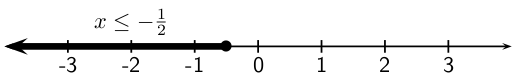
\includegraphics[width=.8\columnwidth]{col11306.imgs/m39254_MG10C10_002.png} % m39254;MG10C10\_002.png;;;6.0;8.5;
\begin{center}
\begin{pspicture}(-4,0.75)(4,1.75)
%\psgrid
\psline[arrows=<->](-4,1)(4,1)
\psdot[dotsize=5pt](-0.5,1)
\multido{\n=-3+1}{7}
{\uput[d](\n,1){$\n$}
\psline(\n,1.1)(\n,0.9)}
\uput[u](-2,1){$x\le-\frac{1}{2}$}
\psline[linewidth=3pt]{->}(-0.5,1)(-4,1)
\end{pspicture}
\end{center}
\vspace{2pt}
\vspace{.1in}
\end{center}
\end{figure}       
\par 

If we represent this answer in interval notation we write $(-\infty ~;-\frac{1}{2}]$.\par
\Note{Assume $x \in \mathbb{R}$ if the set of numbers to be used is not specified.}
Soos jy kan sien, vir die vergelyking is daar slegs ’n enkele waarde van  $x$ waarvoor die vergelyking waar is. Vir
die ongelykheid is daar egter ’n hele versameling waardes waarvoor die ongelykheid waar is. Dit is die groot
verskil tussen gewone vergelykings (gelykhede) en ongelykhede.\par 

\setcounter{subfigure}{0}
\begin{figure}[H] % horizontal\label{m39254*inequalities-1}
\textnormal{Khan academy video on inequalities - 1}\vspace{.1in} \nopagebreak
\label{m39254*yt-media4}\label{m39254*yt-video4}
\raisebox{-5 pt}{ 
\includegraphics[width=0.5cm]{col11306.imgs/summary_www.png}} { (Video:  MG10074 )}
\vspace{2pt}
\vspace{.1in}
\end{figure}    

\setcounter{subfigure}{0}
\begin{figure}[H] % horizontal\label{m39254*inequalities-2}
\textnormal{Khan academy video on inequalities - 2}\vspace{.1in} \nopagebreak
\label{m39254*yt-media5}\label{m39254*yt-video5}
\raisebox{-5 pt}{ 
\includegraphics[width=0.5cm]{col11306.imgs/summary_www.png}} { (Video:  MG10075 )}
\vspace{2pt}
\vspace{.1in}
\end{figure}  
  
\begin{wex}
{Lineêre Ongelykhede }
{
Los op vir $r$: $6-r>2$ \\
Stel jou antwoord op ’n getallelyn voor en in interval notation.}
{ 
\westep{Rearrange and solve for $r$}  
\begin{equation*}
\begin{array}{ccl}\hfill -r&>&2-6\\ \hfill -r&>&-4\end{array}
\end{equation*}
\westep{Wanneer jy met ’n negatiewe getal vermenigvuldig, draai die rigting
van die ongelykheid om.}

\begin{equation*}
r<4
\end{equation*}
(Remember: when you multiply by a minus sign, the direction of the inequality changes.)

\westep{stel die oplossing voor op ’n getallelyn.}

\setcounter{subfigure}{0}
\begin{figure}[H] % horizontal\label{m39254*id157937}
\begin{center}

%\includegraphics{col11306.imgs/m39254_MG10C10
% _003.png} % ;MG10C10\_003.png;;;6.0;8.5;
\begin{center}
\begin{pspicture}(-1,0.4)(6,1.6)
%\psgrid
\psline[arrows=<->](-1,1)(6,1)
\multido{\n=0+1}{6}
{\uput[d](\n,1){$\n$}
\psline(\n,1.1)(\n,0.9)}
\uput[u](2,1){$r<4$}
\psline[linewidth=3pt]{->}(4,1)(-1,1)
\psdot[dotsize=5pt,dotstyle=o](4,1)
\end{pspicture}
\end{center}
}
\vspace{2pt}
\vspace{.1in}
\end{center}
\end{figure}    

\westep{Represent answer in interval notation}
\begin{equation*}
(- \infty~;~4)   
\end{equation*}
}
\end{wex}

\begin{wex}{Solving linear inequalities }
{
Solve for $q$: $4q+3<2(q+3)$ \\
Represent answer on a number line and in interval notation.
}
{
\westep{Brei die hakkies uit}  
\begin{equation*}
\begin{array}{ccl}\hfill 4q+3& <& 2(q+3)\hfill \\ \hfill 4q+3& <& 2q+6\hfill \end{array}
\end{equation*}

\westep{Rearrange and solve for $q$}
\begin{equation*}
\begin{array}{ccl}\hfill 4q+3& <& 2q+6\hfill \\ \hfill 4q-2q& <& 6-3\hfill \\ \hfill 2q& <& 3\hfill \end{array}
\end{equation*}


\westep{deel beide kante deur $2$}  
\begin{equation*}
\begin{array}{ccccc}\hfill 2q& <& 3\hfill &  \\ \hfill q& <& \frac{3}{2}\hfill & \end{array}
\end{equation*}

\westep{stel die oplossing voor op ’n getallelyn} 

\setcounter{subfigure}{0}
\begin{figure}[H] % horizontal\label{m39254*id158287}
\begin{center}
\label{m39254*id158287!!!underscore!!!media}\label{m39254*id158287!!!underscore!!!printimage}
%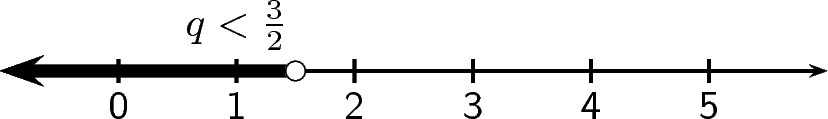
\includegraphics{col11306.imgs/m39254_MG10C10_004.png} % ;MG10C10\_004.png;;;6.0;8.5;
\begin{center}
\begin{pspicture}(-1,0.4)(6,1.6)
%\psgrid
\psline[arrows=<->](-1,1)(6,1)
\multido{\n=0+1}{6}
{\uput[d](\n,1){$\n$}
\psline(\n,1.1)(\n,0.9)}
\uput[u](1,1){$q<\frac{3}{2}$}
\psline[linewidth=3pt]{->}(1.5,1)(-1,1)
\psdot[dotsize=5pt,dotstyle=o](1.5,1)
\end{pspicture}
\end{center}

\vspace{2pt}
\vspace{.1in}
\end{center}
\end{figure}   

\westep{Represent answer in interval notation}
\begin{equation*}
(- \infty~;~\frac{3}{2})
\end{equation*}
}
\end{wex}


\begin{wex}
{Solving compound linear inequalities }
{Solve for $x$: $5\leq x+3<8$ \\
Represent answer on a number line and in interval notation.}  
{
\westep{Subtract $3$ from all terms}
\begin{equation*}
\begin{array}{cccll}\hfill 5-3 &\leq& x+3-3 &<& 8-3\hfill \\
		  \hfill 2&\leq& x &<&5 \hfill
\end{array}
\end{equation*}

\westep{stel die oplossing voor op ’n getallelyn.}

\setcounter{subfigure}{0}
\begin{figure}[H] % horizontal\label{m39254*id158459}
\begin{center}
\label{m39254*id158459!!!underscore!!!media}\label{m39254*id158459!!!underscore!!!printimage}
%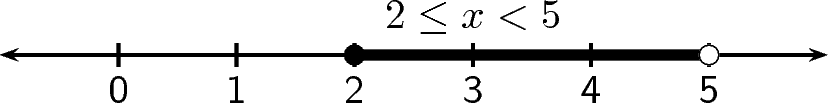
\includegraphics{col11306.imgs/m39254_MG10C10_005.png} % ;MG10C10\_005.png;;;6.0;8.5;
\begin{center}
\begin{pspicture}(-1,0.4)(6,1.6)
%\psgrid
\psline[arrows=<->](-1,1)(6,1)
\multido{\n=0+1}{6}
{\uput[d](\n,1){$\n$}
\psline(\n,1.1)(\n,0.9)}
\uput[u](3,1){$2\le x < 5$}
\psline[linewidth=2.5pt](2,1)(5,1)
\psdot[dotsize=5pt,dotstyle=o](5,1)
\psdot[dotsize=5pt](2,1)
\end{pspicture}
\end{center}

\vspace{2pt}
\vspace{.1in}
\end{center}
\end{figure}       
}

\westep{Represent answer in interval notation}
\begin{equation*}
[~2~;~5)
\end{equation*}
\end{wex}


\begin{exercises}{ }
{
Solve for $x$ and represent the answer on a number line and in interval notation:
\begin{enumerate}[noitemsep, label=\textbf{\arabic*}. ] 

    \item $3x+4>5x+8$
    \item $3(x-1)-2\leq 6x+4$ \vspace{5pt}
    \item $\dfrac{x-7}{3}>\dfrac{2x-3}{2}$\vspace{5pt}
    \item $-4(x-1)<x+2$\vspace{5pt}
    \item $\dfrac{1}{2}x+\dfrac{1}{3}(x-1)\geq \dfrac{5}{6}x-\dfrac{1}{3}$ \vspace{5pt}
    \item $-2\leq x-1<3$ 
    \item $-5<2x-3\leq7$ 
\item $7(3x+2)-5(2x-3)>7$
    \end{enumerate}


\par \raisebox{-0.2em}{
\includegraphics[height=1em]{../icons/www.eps}} Find the answers with the shortcodes:
\par \begin{tabular}[h]{cccccc}
(1.) lcJ  &  (2.) lcS  &  (3.) lch  & \end{tabular}
}
\end{exercises}

\Opsomming
\nopagebreak
\label{m39263} $ \hspace{-5pt}\begin{array}{cccccccccccc}   \end{array} $ \hspace{2 pt}\raisebox{-0.2em}{
\includegraphics[height=1em]{../icons/www.eps}} {(section shortcode: MG10080 )} \par 

\begin{itemize}[noitemsep]
\item ’n Lineêre vergelyking is ’n vergelyking waar die hoogste mag van die veranderlike $1$. is. ’n Lineêre vergelyking het op die meeste een oplossing.
\item ’n Kwadratiese vergelyking is ’n vergelyking waar die hoogste mag van die veranderlike $2$. is. ’n Kwadratiese
vergelyking het op die meeste 2 oplossings
\item ’n Lineêre ongelykheid is soorgelyk aan ’n lineêre vergelyking en met die hoogste mag van die veranderlike
gelyk aan $1$.
\item Wanneer jy weerskante van ’n ongelykheid deel of vermenigvuldig met ’n negatiewe getal,
draai die rigting van die ongelykheid om. 
\item Wanneer 2 onbekende veranderlikes opgelos moet word, moet jy 2 vergelyking gebruik en hierdie verge-
lykings staan bekend as gelyktydige vergelykings. Daar is twee maniere waarop jy gelyktydige lineêre
vergelykings kan oplos: grafies en algebraïes.Om die vergelykings grafies op te los, trek jy ’n grafiek
van elke vergelyking en die oplossing sal die koördinate van die snypunt van die grafieke wees. Om die
oplossing algebraïes te vind, los jy een vergelyking op vir een veranderlike en stel dan daardie oplossing
in die ander vergelyking in om die ander veranderlike se waarde te vind.
\item Lettervergelykings is vergelykings waar jy verskeie letters (veranderlikes) het en jy herrangskik die verge-
lyking om die oplossing te vind in terme van een van die letters (veranderlikes)
\item Wiskundige modellering is waar ons ’n vergelyking of ’n stel vergelykings opstel om ’n probleem wiskundig
voor te stel. Die oplossing van die vergelykings gee dan die oplossing van die probleem.
\end{itemize}

\begin{eocexercises}{}
{
 los op:
\begin{enumerate}[noitemsep, label=\textbf{\arabic*}. ] 
\begin{multicols}{2} 
\item $2(p-1) = 3(p+2)$
\item $3-6k = 2k-1$
\item $m + 6(-m+1) + 5m = 0$
\item $2k + 3 = 2-3(k+3)$
\item $5t-1=t^{2}-(t+2)(t-2)$\vspace{5pt}
\item $3+\dfrac{q}{5} = \dfrac{q}{2}$ \vspace{5pt}
\item $5-\dfrac{2(m+4)}{m} = \dfrac{7}{m}$\vspace{5pt}
\item $\dfrac{2}{t} - 2 - \dfrac{1}{2} = \dfrac{1}{2}(1+\dfrac{2}{t})$\vspace{5pt}
\item $x^{2} - 3x + 2=0$
\item $y^{2} + y = 6$
\item $0=2x^{2} - 5x - 18$\vspace{5pt}
\item $(d+4)(d-3)-d=(3d-2)^{2} - 8d(d-1)$\vspace{5pt}
\item $5x+2\leq4(2x-1)$\vspace{5pt}
\item $\dfrac{4x-2}{6} > 2x+1$\vspace{5pt}
\item $\dfrac{x}{3} - 14 > 14 - \dfrac{x}{7}$\vspace{5pt}
\item $\dfrac{1-a}{2} - \dfrac{2-a}{3} \geq 1$\vspace{5pt}
\item $-5 \leq 2k + 1 < 5$\vspace{5pt}
\item $x-1=\dfrac{42}{x}$  
\end{multicols}
\end{enumerate}

Oplos van lettervergelykings:
\begin{enumerate}[noitemsep, label=\textbf{\arabic*}. ] 
\setcounter{enumi}{18}
\item Los op vir$i$: $P = VI$
\item Los op vir $m$: $E=mc^{2}$
\item Los op vir $t$: $v = u + at$\vspace{5pt}
\item Los op vir $f$: $\dfrac{1}{u} + \dfrac{1}{v} = \dfrac{1}{f}$\vspace{5pt}
\item Los op vir $C$: $F=\frac{9}{5}C + 32$\vspace{5pt}
\item Los op vir $y$: $m = \dfrac{y-c}{x}$\vspace{5pt}
\end{enumerate}

Oplos van gelyktydige vergelykings:
\begin{enumerate}[noitemsep, label=\textbf{\arabic*}. ] 
\setcounter{enumi}{24}
\item $7x+3y=13$ en $2x-3y=-4$  
\item $10=2x+y$ en $y=x-2$
\item $7x-41=3y$ en $17=3x-y$
\item $2y=x+8$ en $4y=2x-44$
\end{enumerate}

Oplos van wiskundige modellering:
\begin{enumerate}[noitemsep, label=\textbf{\arabic*}. ] 
\setcounter{enumi}{28}
\item $\frac{7}{8}$ van ’n getal is $5$ more than of $\frac{1}{3}$  meer as ’n derde van die getal. Vind die getal.
\item Drie liniale en twee penne kos saam R $21,00$. Een liniaal en een pen kos saam R $8,00$. Hoeveel kos ’n pen op sy eie en hoeveel kos ’n liniaal op
sy eie? 
\item ’n Man hardloop na ’n telefoon en terug in $15$ minute. Sy spoed na die telefoon is $5$ km/h en sy spoed terug is $4$ km/h. Wat is die afstand na die foon?.
\item Zanele and Piet skate towards each other on a straight path. They set off $20$ km apart. Zanele skates at $15$ km/h and Piet at $10$ km/h. How far will Piet have skated when they reach each other?
\item When the price of chocolates is increased by R $10$, we can buy five fewer chocolates for R $300$. What was the price of each chocolate before the price was increased?
   
\end{enumerate}
\end{enumerate}

\par \raisebox{-0.2em}{
\includegraphics[height=1em]{../icons/www.eps}} Find the answers with the shortcodes:
\par \begin{tabular}[h]{cccccc}
(1.) lcG  &  (2.) lc7  &  (3.) lcA  &  (4.) lco  &  (5.) lcs  &  (6.) lcH  &  (7.) lc6  &  (8.) lcF  &  (9.) lcL  &  (10.) lcM  & \end{tabular}
}
\end{eocexercises}